\documentclass[11pt]{article}
\usepackage{certmachine}
%% generated by tools/paper-numbers/digits-not-evidence.js from families/oeis-closedform.js over corpus/oeis-constants.json, families/ramanujan-audit.js over corpus/sources/ (PINS.json), instruments/cf/battery.js, ledger.json — do not edit (git be82e126bc6b)
\newcommand{\RepoCommit}{be82e126bc6b}
\newcommand{\DoubleDigits}{15.95}
\newcommand{\OeisSource}{OEIS names.gz + stripped.gz bulk downloads}
\newcommand{\OeisPinned}{2026-08-24}
\newcommand{\ScreenDigits}{17}
\newcommand{\VocabSize}{3{,}763}
\newcommand{\OeisEntries}{14{,}677}
\newcommand{\OeisAudited}{14{,}601}
\newcommand{\OeisSkipped}{76}
\newcommand{\FormsTested}{3{,}742}
\newcommand{\FormsUntested}{21}
\newcommand{\DoubleRefuted}{54{,}636{,}044}
\newcommand{\DoubleRefutedM}{54.6}
\newcommand{\DoubleTestedTotal}{54{,}636{,}942}
\newcommand{\OeisOnRecord}{877}
\newcommand{\OeisHits}{0}
\newcommand{\OeisOpen}{0}
\newcommand{\ImpConstants}{5}
\newcommand{\ImpCount}{21}
\newcommand{\ImpDeepest}{62}
\newcommand{\ImpShallowest}{16}
\newcommand{\ImpSeconds}{12}
\newcommand{\EvilClass}{$2$, $20$, $\tfrac{1}{5}$}
\newcommand{\EvilDepth}{62}
\newcommand{\EvilPublished}{105}
\newcommand{\EvilPrefix}{0}
\newcommand{\EvilGapMant}{$2.17\times10^{-63}$}
\newcommand{\EvilGapRel}{$1.08\times10^{-63}$}
\newcommand{\EvilGapProb}{$2.17\times10^{-64}$}
\newcommand{\EvilSpellings}{6}
\newcommand{\EvilNines}{62}
\newcommand{\EvilAfter}{783377}
\newcommand{\EvilLead}{1}
\newcommand{\RamDepth}{16}
\newcommand{\RamPublished}{105}
\newcommand{\ImpAtScreen}{2}
\newcommand{\ImpAtScreenIds}{\texttt{A226120} and \texttt{A266296}}
\newcommand{\FiveRows}{\texttt{A271880} & 105 & \texttt{Decimal expansion of the probability that a random real number is evil.} \\
\texttt{A181284} & 105 & \texttt{Decimal expansion of sqrt(9/121 * 100\textasciicircum{}m + (112 - 44*m)/121), where m=30.} \\
\texttt{A359187} & 87 & \texttt{Decimal expansion of the real part of (-sqrt(2))\textasciicircum{}\textasciicircum{}9, where \textasciicircum{}\textasciicircum{} indicates tetration or hyper-4 (e.g., 2\textasciicircum{}\textasciicircum{}4 = 2\textasciicircum{}(2\textasciicircum{}(2\textasciicircum{}2))).} \\
\texttt{A226120} & 100 & \texttt{Decimal expansion of Sum\_\{n$\ge$1\} n\textasciicircum{}3/(exp(2*Pi*n/7)-1).} \\
\texttt{A266296} & 105 & \texttt{Decimal expansion of a number close to 24, related to the Ramanujan number e\textasciicircum{}(Pi*sqrt(163)).} \\}
\newcommand{\ImpostorRows}{\texttt{A271880} & $2$ & \texttt{2/1}, \texttt{sqrt(4/1)}, \texttt{cbrt(8/1)}, \texttt{sqrt2\textasciicircum{}(2/1)} & 0 & 62 & 105 & refuted \\
\texttt{A271880} & $20$ & \texttt{20/1} & 0 & 62 & 105 & refuted \\
\texttt{A271880} & $\tfrac{1}{5}$ & \texttt{1/5} & 0 & 62 & 105 & refuted \\
\texttt{A181284} & $\tfrac{3}{11}$ & \texttt{3/11} & 58 & 58 & 105 & refuted \\
\texttt{A181284} & $\tfrac{30}{11}$ & \texttt{30/11} & 58 & 58 & 105 & refuted \\
\texttt{A359187} & $1$ & \texttt{1/1}, \texttt{sqrt(1/1)}, \texttt{cbrt(1/1)} & 45 & 44 & 87 & refuted \\
\texttt{A359187} & $10$ & \texttt{10/1} & 45 & 44 & 87 & refuted \\
\texttt{A359187} & $\tfrac{1}{10}$ & \texttt{1/10} & 45 & 44 & 87 & refuted \\
\texttt{A226120} & $1$ & \texttt{1/1}, \texttt{sqrt(1/1)}, \texttt{cbrt(1/1)} & 17 & 16 & 100 & refuted \\
\texttt{A226120} & $10$ & \texttt{10/1} & 17 & 16 & 100 & refuted \\
\texttt{A226120} & $\tfrac{1}{10}$ & \texttt{1/10} & 17 & 16 & 100 & refuted \\
\texttt{A266296} & $24$ & \texttt{24/1} & 16 & 16 & 105 & refuted \\
\texttt{A266296} & $\tfrac{12}{5}$ & \texttt{12/5} & 16 & 16 & 105 & refuted \\
\texttt{A266296} & $\tfrac{6}{25}$ & \texttt{6/25} & 16 & 16 & 105 & refuted \\}
\newcommand{\CalibCount}{8}
\newcommand{\RmSeconds}{6}
\newcommand{\RmPrinted}{51}
\newcommand{\RmSurvive}{50}
\newcommand{\RmRefuted}{1}
\newcommand{\RmFlagship}{39}
\newcommand{\RmFlagshipSurvive}{38}
\newcommand{\RmWidest}{$1.16\times10^{-12}$}
\newcommand{\RmWidestId}{\texttt{rm-cat-04}}
\newcommand{\RmWidestForm}{720/(450G-299)}
\newcommand{\RmNarrowest}{$2.22\times10^{-16}$}
\newcommand{\RmSheets}{7}
\newcommand{\RmKnown}{10}
\newcommand{\RmProven}{2}
\newcommand{\RmSameValuePairs}{4}
\newcommand{\RmSameValueList}{\texttt{rm-e-a}/\texttt{rm-e-b}, \texttt{rm-cat-02}/\texttt{rm-cat-05}, \texttt{rm-cat-03}/\texttt{rm-cat-10}, \texttt{rm-cat-07}/\texttt{rm-cat-11}}
\newcommand{\PinRows}{$e$ (2018) & 13 & 3 & \texttt{ebbf12b7839844da\ldots} \\
$\pi$ (2018) & 15 & 2 & \texttt{48b35cb010dc58f5\ldots} \\
$\zeta(3)$ (2020) & 5 & 5 & \texttt{6429e280dad89fd3\ldots} \\
Catalan $G$ (2020) & 23 & 23 & \texttt{8267938820519d4b\ldots} \\
$\pi^2$ (2021) & 12 & 12 & \texttt{9d7154cdf28052fd\ldots} \\
$\ln 2$ (2020) & 1 & 1 & \texttt{479ce83bc248a029\ldots} \\
mixed $\zeta$ orders (2022) & 5 & 5 & \texttt{c7eaafbad08058ff\ldots} \\}
\newcommand{\EDisplays}{13}
\newcommand{\PiDisplays}{15}
\newcommand{\ERows}{3}
\newcommand{\PiRows}{2}
\newcommand{\TableRows}{46}
\newcommand{\RmListed}{10}
\newcommand{\RmOutside}{3}
\newcommand{\RmOutsideList}{\texttt{results\_\allowbreak{}pi\_\allowbreak{}4521\_\allowbreak{}050418.pdf}, \texttt{results\_\allowbreak{}pi\_\allowbreak{}5411\_\allowbreak{}220318.pdf}, \texttt{results\_\allowbreak{}5717\_\allowbreak{}200418\_\allowbreak{}filtered.pdf}}
\newcommand{\RmSweepDate}{2026-10-07}
\newcommand{\ZetaThreeK}{6{,}000}
\newcommand{\ZetaThreeWidth}{$9.65\times10^{-17}$}
\newcommand{\ZetaThreeLo}{1.2020569031595942}
\newcommand{\ZetaThreeHi}{1.2020569031595945}
\newcommand{\ZetaFiveWidth}{$3.3\times10^{-21}$}
\newcommand{\ZetaSevenWidth}{$1.1\times10^{-27}$}
\newcommand{\ZetaHighK}{2{,}000}
\newcommand{\CatalanWidth}{$1.2\times10^{-18}$}
\newcommand{\PiSqWidth}{$5.1\times10^{-57}$}
\newcommand{\LnTwoWidth}{$1.6\times10^{-58}$}
\newcommand{\CatalanEWidth}{$9.3\times10^{-18}$}
\newcommand{\CatalanConvexity}{96k^2+288k+184}
\newcommand{\ZetaThreeRows}{\texttt{rm-z3-pos} & known & $5/(2\zeta(3))$ & $[2.079768431451768,\ 2.079768431451769]$ & $8.88\times10^{-16}$ & 120 \\
\texttt{rm-z3-inv} & known & $1/\zeta(3)$ & $[0.831907372580699,\ 0.831907372580719]$ & $2.01\times10^{-14}$ & 10000000 \\
\texttt{rm-z3-apery} & known (Ap\'ery) & $6/\zeta(3)$ & $[4.991444235484244,\ 4.991444235484246]$ & $1.78\times10^{-15}$ & 60 \\
\texttt{rm-z3-new1} & unproven & $8/(7\zeta(3))$ & $[0.950751282949380,\ 0.950751282949380]$ & $2.22\times10^{-16}$ & 60 \\
\texttt{rm-z3-new2} & unproven & $12/(7\zeta(3))$ & $[1.426126924424070,\ 1.426126924424070]$ & $8.88\times10^{-16}$ & 80 \\}
\newcommand{\ZetaThreePosRow}{\texttt{rm-z3-pos}}
\newcommand{\InvWidth}{$2.01\times10^{-14}$}
\newcommand{\InvDepth}{$10^{7}$}
\newcommand{\InvBandL}{n^{3}+2n^{2}}
\newcommand{\InvBandU}{2n^{3}+3n^{2}+3n+1}
\newcommand{\AperyNZero}{52}
\newcommand{\AperyL}{33n^{3}}
\newcommand{\AperyU}{35n^{3}}
\newcommand{\AperyDepth}{60}
\newcommand{\AperyChecks}{\item a(n) $>$ 0 for all n $\ge$ 1
\item L(n) $>$ 0 for all n $\ge$ 52
\item (T) b(n) $-$ L(n) $\ge$ 0 for all n $\ge$ 52 (shift-and-check coefficient positivity)
\item (T) U(n) $-$ b(n) $\ge$ 0 for all n $\ge$ 52 (shift-and-check coefficient positivity)
\item (I$-$) band invariance from below for all n $\ge$ 52 (shift-and-check coefficient positivity)
\item (I+) band invariance from above for all n $\ge$ 52 (shift-and-check coefficient positivity)}
\newcommand{\AperyWidth}{$1.78\times10^{-15}$}
\newcommand{\FastDepth}{80}
\newcommand{\SpuriousIdentity}{holds}
\newcommand{\InvBandRows}{$n^{3}$ & certified; evaluation refused (tail interval contains 0 at level 968) \\
$n^{3}+n^{2}$ & certified; enclosure $[0.831907,\ 0.831907]$, width $1.7\times10^{-11}$ \\
$n^{3}+2n^{2}$ & certified; enclosure $[0.831907,\ 0.831907]$, width $8.7\times10^{-12}$ \\
$n^{3}+3n^{2}$ & refused: (I$-$) band invariance from below FAILS \\}
\newcommand{\InvProbeDepth}{200{,}000}
\newcommand{\InvBandC}{2}
\newcommand{\BranchRows}{\texttt{rm-zo-z4z2} & 4 & $\alpha^2-3\alpha-4$ & $(\alpha-4)(\alpha+1)$ & $n^{4}+4n^{3}$ & $8.88\times10^{-16}$ \\
\texttt{rm-zo-z5z3a} & 5 & $\alpha^2-4\alpha-12$ & $(\alpha-6)(\alpha+2)$ & $n^{5}+6n^{4}$ & $1.78\times10^{-15}$ \\
\texttt{rm-zo-z5z3b-printed} & 5 & $\alpha^2-4\alpha-12$ & $(\alpha-6)(\alpha+2)$ & $n^{5}+6n^{4}$ & $8.88\times10^{-16}$ \\
\texttt{rm-zo-z5z3c} & 5 & $\alpha^2-4\alpha-32$ & $(\alpha-8)(\alpha+4)$ & $n^{5}+8n^{4}$ & $3.55\times10^{-15}$ \\
\texttt{rm-zo-z7z3} & 7 & $\alpha^2-6\alpha-16$ & $(\alpha-8)(\alpha+2)$ & $n^{7}+8n^{6}$ & $1.78\times10^{-15}$ \\}
\newcommand{\RowThreePoly}{2n^{5}+5n^{4}+22n^{3}+28n^{2}+15n+3}
\newcommand{\RowThreeAOne}{75}
\newcommand{\RowThreePrintedAOne}{275}
\newcommand{\RowThreePrintedValue}{-1.5035}
\newcommand{\RowThreeEnclosure}{[2.9862258661092707,\ 2.9862258661092715]}
\newcommand{\RowThreeWidth}{$8.88\times10^{-16}$}
\newcommand{\RowThreeFormWidth}{$2.18\times10^{-16}$}
\newcommand{\RowThreeCorrFormWidth}{$8.60\times10^{-16}$}
\newcommand{\RowThreeDepth}{200{,}000}
\newcommand{\RowThreeCF}{2.986225866109}
\newcommand{\RmTwoKLeading}{\texttt{rm-e-a} ($a_0=0$), \texttt{rm-e-b} ($a_0=0$), \texttt{rm-e-c} ($a_0=1$), \texttt{rm-pi-a} ($a_0=0$), \texttt{rm-pi-b} ($a_0=0$)}
\newcommand{\RegistryRowsA}{\multicolumn{7}{l}{\emph{$e$ (2018), \texttt{results\_e\_4614\_070418.pdf}}} \\
\texttt{rm-e-a} & known & $2n$ & $1;\,4n-4$ & $e/2-1$ & survives & $3.9\times10^{-16}$ \\
\texttt{rm-e-b} & known & $n+1$ & $1;\,n+1$ & $e/2-1$ & survives & $3.9\times10^{-16}$ \\
\texttt{rm-e-c} & known & $n+1$ & $n+1$ & $e-1$ & survives & $8.9\times10^{-16}$ \\
\multicolumn{7}{l}{\emph{$\pi$ (2018), \texttt{results\_pi\_0101\_060418.pdf}}} \\
\texttt{rm-pi-a} & known & $2n-1$ & $1;\,n^{2}-2n+1$ & $\pi/4$ & survives & $7.8\times10^{-16}$ \\
\texttt{rm-pi-b} & known & $2n+1$ & $1;\,n^{2}-1$ & $\pi/4-1/2$ & survives & $3.9\times10^{-16}$ \\
\multicolumn{7}{l}{\emph{$\zeta(3)$ (2020), \texttt{rm\_zeta3.pdf}}} \\
\texttt{rm-z3-pos} & known & $3n^{3}+10n^{2}+8n+2$ & $4n^{6}-2n^{5}$ & $5/(2\zeta(3))$ & survives & $8.9\times10^{-16}$ \\
\texttt{rm-z3-inv} & known & $2n^{3}+3n^{2}+3n+1$ & $-n^{6}$ & $1/\zeta(3)$ & survives & $2.0\times10^{-14}$ \\
\texttt{rm-z3-apery} & known (Ap\'ery) & $34n^{3}+51n^{2}+27n+5$ & $-n^{6}$ & $6/\zeta(3)$ & survives & $1.8\times10^{-15}$ \\
\texttt{rm-z3-new1} & unproven & $6n^{3}+9n^{2}+5n+1$ & $-n^{6}$ & $8/(7\zeta(3))$ & survives & $2.2\times10^{-16}$ \\
\texttt{rm-z3-new2} & unproven & $10n^{3}+15n^{2}+9n+2$ & $-16n^{6}$ & $12/(7\zeta(3))$ & survives & $8.9\times10^{-16}$ \\
\multicolumn{7}{l}{\emph{$\ln 2$ (2020), \texttt{rm\_other.pdf}}} \\
\texttt{rm-ln2} & unproven & $3n^{2}+7n+4$ & $-(2n^{4}+4n^{3}+2n^{2})$ & $1/(-\log2+1)$ & survives & $1.8\times10^{-15}$ \\
\multicolumn{7}{l}{\emph{mixed $\zeta$ orders (2022), \texttt{rm\_zeta\_orders.pdf}}} \\
\texttt{rm-zo-z4z2} & unproven & \begin{tabular}[t]{@{}l@{}}$2n^{4}+4n^{3}$\\$+10n^{2}+8n+3$\end{tabular} & $-n^{8}$ & $-1/(\zeta(4)+4\zeta(2)-8)$ & survives & $8.9\times10^{-16}$ \\
\texttt{rm-zo-z5z3a} & unproven & \begin{tabular}[t]{@{}l@{}}$2n^{5}+5n^{4}+22n^{3}$\\$+28n^{2}+23n+7$\end{tabular} & $-n^{10}$ & $2/(2\zeta(5)+6\zeta(3)-9)$ & survives & $1.8\times10^{-15}$ \\
\texttt{rm-zo-z5z3b-printed} & printed & \begin{tabular}[t]{@{}l@{}}$2n^{5}+5n^{4}+22n^{3}$\\$+28n^{2}+15n+3$\end{tabular} & $-n^{10}$ & $2/(2\zeta(5)-2\zeta(3)-1)$ & \textbf{refuted} & $8.9\times10^{-16}$ \\
\texttt{rm-zo-z5z3b-corrected} & ours & \begin{tabular}[t]{@{}l@{}}$2n^{5}+5n^{4}+22n^{3}$\\$+28n^{2}+15n+3$\end{tabular} & $-n^{10}$ & $2/(2\zeta(5)-2\zeta(3)+1)$ & survives (ours) & $8.9\times10^{-16}$ \\
\texttt{rm-zo-z5z3c} & unproven & \begin{tabular}[t]{@{}l@{}}$2n^{5}+5n^{4}+42n^{3}$\\$+58n^{2}+45n+13$\end{tabular} & $-n^{10}$ & $64/(64\zeta(5)+176\zeta(3)-273)$ & survives & $3.6\times10^{-15}$ \\
\texttt{rm-zo-z7z3} & unproven & \begin{tabular}[t]{@{}l@{}}$2n^{7}+7n^{6}+37n^{5}+75n^{4}$\\$+99n^{3}+77n^{2}+31n+5$\end{tabular} & $-n^{14}$ & $1/(\zeta(7)-4\zeta(3)+4)$ & survives & $1.8\times10^{-15}$ \\}
\newcommand{\RegistryRowsB}{\multicolumn{7}{l}{\emph{Catalan $G$ (2020), \texttt{rm\_catalan.pdf}}} \\
\texttt{rm-cat-known} & known & $10n^{2}+7n+2$ & $-(16n^{4}-24n^{3}+12n^{2}-2n)$ & $6/((8G-\pi\operatorname{arcosh}2))$ & survives & $2.2\times10^{-15}$ \\
\texttt{rm-cat-01} & unproven & $3n^{2}+3n+1$ & $-2n^{4}$ & $1/(2G)$ & survives & $8.9\times10^{-16}$ \\
\texttt{rm-cat-02} & unproven & $3n^{2}+3n+1$ & $-(2n^{4}+2n^{3})$ & $2/(2G-1)$ & survives & $8.3\times10^{-14}$ \\
\texttt{rm-cat-03} & unproven & $3n^{2}+3n+1$ & $-(2n^{4}+4n^{3})$ & $24/(18G-11)$ & survives & $4.5\times10^{-13}$ \\
\texttt{rm-cat-04} & unproven & $3n^{2}+3n+1$ & $-(2n^{4}+6n^{3})$ & $720/(450G-299)$ & survives & $1.2\times10^{-12}$ \\
\texttt{rm-cat-05} & unproven & $3n^{2}+7n+3$ & $-(2n^{4}+4n^{3})$ & $2/(2G-1)$ & survives & $1.3\times10^{-15}$ \\
\texttt{rm-cat-06} & unproven & $3n^{2}+7n+3$ & $-(2n^{4}+6n^{3}+4n^{2})$ & $4/(2G+1)$ & survives & $3.3\times10^{-15}$ \\
\texttt{rm-cat-07} & unproven & $3n^{2}+7n+3$ & $-(2n^{4}+8n^{3}+8n^{2})$ & $16/(6G-1)$ & survives & $9.3\times10^{-14}$ \\
\texttt{rm-cat-08} & unproven & $3n^{2}+7n+3$ & $-(2n^{4}+10n^{3}+12n^{2})$ & $288/(90G-31)$ & survives & $3.3\times10^{-13}$ \\
\texttt{rm-cat-09} & unproven & $3n^{2}+9n+7$ & $-(2n^{4}+6n^{3}+6n^{2}+2n)$ & $1/(-2G+2)$ & survives & $3.6\times10^{-15}$ \\
\texttt{rm-cat-10} & unproven & $3n^{2}+11n+5$ & $-(2n^{4}+8n^{3})$ & $24/(18G-11)$ & survives & $1.8\times10^{-15}$ \\
\texttt{rm-cat-11} & unproven & $3n^{2}+11n+5$ & $-(2n^{4}+10n^{3}+8n^{2})$ & $16/(6G-1)$ & survives & $2.2\times10^{-15}$ \\
\texttt{rm-cat-12} & unproven & $3n^{2}+11n+5$ & $-(2n^{4}+12n^{3}+16n^{2})$ & $64/(18G+13)$ & survives & $7.5\times10^{-15}$ \\
\texttt{rm-cat-13} & unproven & $3n^{2}+11n+9$ & $-(2n^{4}+8n^{3}+8n^{2})$ & $4/(6G-5)$ & survives & $5.3\times10^{-15}$ \\
\texttt{rm-cat-14} & unproven & $3n^{2}+11n+9$ & $-(2n^{4}+10n^{3}+16n^{2}+8n)$ & $8/(-2G+3)$ & survives & $3.6\times10^{-15}$ \\
\texttt{rm-cat-15} & unproven & $3n^{2}+11n+9$ & $-(2n^{4}+12n^{3}+24n^{2}+16n)$ & $32/(2G+5)$ & survives & $1.2\times10^{-14}$ \\
\texttt{rm-cat-16} & unproven & $3n^{2}+11n+9$ & $-(2n^{4}+14n^{3}+32n^{2}+24n)$ & $192/(18G+13)$ & survives & $9.1\times10^{-14}$ \\
\texttt{rm-cat-17} & unproven & $3n^{2}+13n+13$ & $-(2n^{4}+10n^{3}+14n^{2}+6n)$ & $6/(-18G+17)$ & survives & $5.3\times10^{-15}$ \\
\texttt{rm-cat-18} & unproven & $3n^{2}+15n+15$ & $-(2n^{4}+12n^{3}+16n^{2})$ & $48/(90G-79)$ & survives & $3.6\times10^{-15}$ \\
\texttt{rm-cat-19} & unproven & $3n^{2}+15n+15$ & $-(2n^{4}+14n^{3}+28n^{2}+16n)$ & $32/(-18G+19)$ & survives & $5.3\times10^{-15}$ \\
\texttt{rm-cat-20} & unproven & $3n^{2}+15n+15$ & $-(2n^{4}+16n^{3}+40n^{2}+32n)$ & $128/(-6G+17)$ & survives & $7.1\times10^{-15}$ \\
\texttt{rm-cat-21} & unproven & $3n^{2}+15n+19$ & $-(2n^{4}+12n^{3}+24n^{2}+16n)$ & $8/(54G-49)$ & survives & $7.1\times10^{-15}$ \\
\texttt{rm-cat-22} & unproven & $3n^{2}+17n+23$ & $-(2n^{4}+14n^{3}+30n^{2}+18n)$ & $12/(-90G+83)$ & survives & $7.1\times10^{-15}$ \\
\multicolumn{7}{l}{\emph{$\pi^2$ (2021), \texttt{rm\_zeta2.pdf}}} \\
\texttt{rm-z2-known} & known & $11n^{2}+11n+3$ & $n^{4}$ & $30/(\pi^{2})$ & survives & $8.9\times10^{-16}$ \\
\texttt{rm-z2-proven1} & proven & $3n^{2}+3n+1$ & $-(2n^{4}-n^{3})$ & $8/(\pi^{2})$ & survives & $1.9\times10^{-15}$ \\
\texttt{rm-z2-new1} & unproven & $3n^{2}+3n+1$ & $-(2n^{4}-3n^{3})$ & $16/(\pi^{2}+4)$ & survives & $4.4\times10^{-15}$ \\
\texttt{rm-z2-new2} & unproven & $7n^{2}+7n+2$ & $8n^{4}$ & $24/(\pi^{2})$ & survives & $1.3\times10^{-15}$ \\
\texttt{rm-z2-proven2} & proven & $5n^{2}+6n+2$ & $-(4n^{4}-2n^{3})$ & $18/(\pi^{2})$ & survives & $1.6\times10^{-15}$ \\
\texttt{rm-z2-new3} & unproven & $3n^{2}+7n+3$ & $-(2n^{4}+3n^{3}-2n^{2})$ & $16/(\pi^{2}-4)$ & survives & $2.7\times10^{-15}$ \\
\texttt{rm-z2-new4} & unproven & $3n^{2}+7n+3$ & $-(2n^{4}+n^{3}-6n^{2})$ & $32/(\pi^{2})$ & survives & $7.1\times10^{-15}$ \\
\texttt{rm-z2-new5} & unproven & $3n^{2}+11n+9$ & $-(2n^{4}+7n^{3}+4n^{2}-4n)$ & $16/(\pi^{2}-8)$ & survives & $7.1\times10^{-15}$ \\
\texttt{rm-z2-new6} & unproven & $3n^{2}+11n+9$ & $-(2n^{4}+9n^{3}+12n^{2}+4n)$ & $16/(-\pi^{2}+12)$ & survives & $2.7\times10^{-15}$ \\
\texttt{rm-z2-new7} & unproven & $3n^{2}+15n+15$ & $-(2n^{4}+13n^{3}+22n^{2}+8n)$ & $32/(-3\pi^{2}+32)$ & survives & $3.6\times10^{-15}$ \\
\texttt{rm-z2-new8} & unproven & $3n^{2}+9n+7$ & $-(2n^{4}+3n^{3}-3n^{2}-7n-3)$ & $(3\pi^{2}+16)/(-\pi^{2}+16)$ & survives & $1.1\times10^{-14}$ \\
\texttt{rm-z2-new9} & unproven & $5n^{2}+14n+10$ & $-(4n^{4}+6n^{3})$ & $18/(\pi^{2}-8)$ & survives & $3.6\times10^{-15}$ \\}
\newcommand{\CfBatteryPass}{38}
\newcommand{\CfBatteryRed}{12}
\newcommand{\CfBatteryCalib}{3}


\theoremstyle{definition}
\newtheorem{definition}{Definition}
\theoremstyle{plain}

\newcommand{\vS}{\textsc{survives}}
\newcommand{\vR}{\textsc{refuted}}
\newcommand{\vF}{\textsc{refused}}
\newcommand{\cf}[1]{\texttt{#1}}

\title{Digit agreement is not evidence:\\
an impostor catalog of published constants refuted in exact arithmetic,\\
and the Ramanujan Machine's printed sheets re-decided}
\author{\cmauthor}
\date{October 2026 --- draft v0.1 for review; every number interpolated from the record; machine-derived, not peer-reviewed; author list to be agreed}

\begin{document}
\maketitle

\begin{abstract}
A decimal match to many digits is the usual evidence offered when a computed value is announced to equal a closed form. This note measures how far that evidence reaches, in both directions, with a re-runnable record. Part~I is the reverse experiment: among the \OeisAudited\ published decimal expansions in the OEIS bulk files, a double-precision screen against \FormsTested\ closed-form spellings leaves \ImpConstants\ constants whose digits agree with simple rationals past the screen's \ScreenDigits\ significant digits, and one integer comparison at the full published length refutes all \ImpCount\ agreeing spellings; the agreement depth, defined exactly in the relative sense, runs from \ImpShallowest\ to \ImpDeepest\ significant digits (\texttt{A271880} agrees with $1/5$ to \EvilDepth\ digits and is not $1/5$). Part~II is the forward experiment: the Ramanujan Machine's seven published result sheets are re-decided as a standing registry of \RmPrinted\ printed continued-fraction rows, each enclosed by a tail band proved inside the certificate and compared with its claimed closed form in exact rational arithmetic against hash-pinned sheet bytes. \RmSurvive\ rows survive at widths between \RmNarrowest\ and \RmWidest; one, the third row of the 2022 mixed-orders sheet, is refuted as printed---a sign slip---and the sign-corrected identity survives on the same enclosure. One grammar serves both parts: a claim \vS\ to a stated width, is \vR\ by a theorem, or is \vF\ with the reason, and every verdict is recomputed from the records at every build. For announcements of machine-found mathematics the conclusion is operational: publish the object and a certificate, not a digit count.
\end{abstract}

\section{Introduction}

Experimental mathematics identifies constants by numerical agreement. A value is computed to high precision, candidate closed forms are generated, and a match to a stated number of digits is reported, with the credibility of the match argued from the precision and the size of the search space \cite{BB04}. Integer-relation algorithms make the search systematic: PSLQ and LLL find an integer relation among given real numbers when one exists at the working precision, and their output is likewise a relation that holds to that precision \cite{FBA99,LLL82}. The method is productive and its practitioners call the output a conjecture. The Ramanujan Machine \cite{RM21} applies the same logic at scale to polynomial continued fractions: a search finds continued fractions whose values agree numerically with closed forms in a fundamental constant, and the result sheets print the matches as conjectures, marking the rows for which ``we have not found any formal proof yet'' as \emph{new and unproven} \cite{RMsheets}.

This note asks a narrow question about such evidence and answers it on the record: how many digits of agreement separate a true identity from a false one? There exist published constants that agree with a simple closed form far past any precision used in practice and are provably not that form, and a screen that accepts digit agreement at any fixed depth accepts them (Part~I, on the OEIS corpus of decimal expansions \cite{OEIS}). And each printed conjecture of the Ramanujan Machine can be decided against a rigorous enclosure of its continued fraction, which either contains the claimed value, to a width that is reported, or provably excludes it (Part~II, on the Machine's seven result sheets).

The methods are elementary and are stated with proofs, because the point is that nothing beyond them is needed: an integer inequality decides a rational form against a digit stream; a backward interval evaluation from a proved tail band encloses a continued fraction; a partial sum with a convexity bound on the tail brackets $\zeta(s)$; the final comparison is made in exact rational arithmetic. What this note adds is not a theorem about any constant but a decision grammar and a public record. Every claim below carries one of three verdicts, \vS\ (the claimed value lies inside a rigorous enclosure of stated width; equality is not proved), \vR\ (the claimed value lies provably outside the enclosure; a theorem), or \vF\ (the instrument cannot decide and says why), and every verdict is recomputed from pinned inputs at every build of the repository that holds this note, by instruments that must first fire their planted controls \cite{repo}. We use \emph{certified} in one sense only: a statement is certified when a program has decided it in exact rational or outward-rounded interval arithmetic from pinned inputs, and the decision is re-run at every build; elsewhere we say decided or proved. Other people's published rows are \emph{re-decided}, a false printed row is reported with its mechanism and, where the computation behind it was right, with the corrected identity decided on the same enclosure, and a survival is never promoted: a row that survives to a width of $10^{-15}$ is a conjecture with a certified numerical consistency, not a theorem.

\section{Statement of results}

\begin{theorem}[the impostor catalog]\label{thm:imp}
Of the \OeisAudited\ OEIS decimal expansions audited (Section~\ref{sec:corpus}), exactly \ImpConstants\ have digit streams consistent, at \ScreenDigits\ significant digits, with at least one rational value among the \FormsTested\ closed-form spellings of the vocabulary; across the five there are \ImpCount\ such spellings. For every one of the \ImpCount, the published digit stream is inconsistent with the spelling's value at the full published length: the integer inequality of Lemma~\ref{lem:exact} fails. Their agreement depths in the sense of Definition~\ref{def:depth} lie between \ImpShallowest\ and \ImpDeepest\ significant digits (Table~\ref{tab:imp}).
\end{theorem}

The refutations are conditional on the published digits being correct, and they are refutations up to a power of ten, since the bulk file carries no decimal point (Section~\ref{sec:corpus}). The same instrument keeps every closed form it is calibrated on (Section~\ref{sec:calib}).

\begin{theorem}[the registry]\label{thm:reg}
Of the \RmPrinted\ printed rows of the Ramanujan Machine's seven result sheets transcribed in Section~\ref{sec:sheets}, \RmSurvive\ \vS: the claimed closed form lies inside a rigorous enclosure of the row's continued fraction, of width between \RmNarrowest\ and \RmWidest, the comparison made in exact rational arithmetic. One row, the third of the July 2022 sheet \emph{Results using mixed orders of $\zeta$}, is \vR\ as printed: the printed identity
\[
\frac{2}{2\zeta(5)-2\zeta(3)-1}\;=\;a_0-\cfrac{1}{a_1-\cfrac{2^{10}}{a_2-\cfrac{3^{10}}{a_3-\cdots}}},\qquad a_n=\RowThreePoly,
\]
is false. The continued fraction defined by the row's own polynomials lies in an enclosure of width \RowThreeWidth\ around $\RowThreeCF$, while the printed left-hand side is $\RowThreePrintedValue\ldots$
\end{theorem}

\begin{proposition}[the correction]\label{prop:corr}
The sign-corrected identity $2/(2\zeta(5)-2\zeta(3)+1)$ \vS\ on the enclosure of Theorem~\ref{thm:reg}: the exact bracket of the corrected value, of width \RowThreeCorrFormWidth, meets the enclosure of width \RowThreeWidth.
\end{proposition}

\section{Part I: the impostor catalog}

\subsection{The corpus and the screen}\label{sec:corpus}

The corpus is the pair of OEIS bulk files \texttt{names.gz} and \texttt{stripped.gz} \cite{OEIS}, fetched on \OeisPinned, restricted to the \OeisEntries\ entries whose name begins ``Decimal expansion of''. The bulk files carry each entry's digit stream but not its offset, so the position of the decimal point is unknown; the family therefore compares \emph{mantissas}, the digit stream read as a number in $[1,10)$, which rules out a form together with all its multiples by powers of ten, a strictly stronger refutation than a placed comparison would give. \OeisSkipped\ entries whose names declare a periodic or characteristic sequence rather than a constant are excluded by a name filter, leaving \OeisAudited.

The closed-form vocabulary is generated, not listed: rationals $p/q$ with $p,q\le32$; square and cube roots of rationals; quadratic irrationals $(a+b\sqrt d)/c$ for $d\in\{2,3,5,6,7,10,13\}$; rational multiples and powers of $\pi$, $e$, $\ln2$, $\ln10$, $\sqrt2$, $\sqrt3$, $\sqrt5$, $\varphi$ and Euler's constant, with products and quotients of pairs of them; and logarithms and exponentials of small rationals, every spelling in lowest terms: \VocabSize\ spellings, of which \FormsUntested\ (logarithms of rationals below one) are negative and never compared with a mantissa, so each constant is screened against \FormsTested.

The screen is a double-precision enclosure of the published mantissa: the first \ScreenDigits\ significant digits define an interval of width $10^{1-\ScreenDigits}$, padded outward by \ScreenUlps\ units in the last place, and a spelling survives when its own mantissa falls inside. Over the corpus this is \DoubleTestedTotal\ comparisons, of which \DoubleRefuted\ refute. Survivors are decided by the entry's own record: \OeisOnRecord\ surviving forms are stated by the entry's name or its fetched formula field (the decimal expansion of $2e$ survives as $2e$), and the audit reports \OeisHits\ discoveries and \OeisOpen\ open candidates. The rational survivors pass to an exact stage, the subject of this part.

\subsection{The exact decision}\label{sec:exact}

\begin{lemma}[rational form against a digit stream]\label{lem:exact}
Let $d_1d_2\cdots d_k$ be the published significant digits of a constant, $d_1\neq0$, and let $D=\sum_{i=1}^k d_i10^{k-i}$ be the stream read as a $k$-digit integer. The published digits assert that the mantissa $m$ of the constant satisfies $D\cdot10^{1-k}\le m<(D+1)\cdot10^{1-k}$. Let $r>0$ be rational and let $P/Q$ be its mantissa, $P,Q$ positive integers with $1\le P/Q<10$. Then $m=P/Q$ is consistent with the published digits if and only if
\begin{equation}\label{eq:exact}
D\,Q\;\le\;P\cdot10^{k-1}\;<\;(D+1)\,Q .
\end{equation}
\end{lemma}
\begin{proof}
Multiply the asserted bounds on $m$ by $Q\cdot10^{k-1}$, a positive integer.
\end{proof}

Every quantity in \eqref{eq:exact} is an integer, so the decision is a comparison of integers; no floating-point number participates, and there is no precision to argue about. A spelling is routed to the exact stage whenever its \emph{value} is rational, however it is spelled ($\sqrt{4/1}$, $\sqrt[3]{8/1}$ and $\sqrt2^{\,2/1}$ are all $2$, and a continued-fraction expansion of the value detects a small denominator in any of them), and a refutation by \eqref{eq:exact} reads ``not equal to $r\cdot10^j$ for any integer $j$, given the published digits''.

\subsection{Agreement depth, and why a prefix count lies}\label{sec:depth}

\begin{definition}[agreement depth]\label{def:depth}
With $D$, $k$, $P$, $Q$ as in Lemma~\ref{lem:exact}, let $I=[D,D+1)\cdot10^{1-k}$ be the published mantissa interval, $m_r=P/Q$ the form's mantissa and $g=\operatorname{dist}(m_r,I)$ their gap, an exact rational. The agreement depth of the form with the published digits is
\[
\delta=\max\{\,d\in\mathbb Z_{\ge0}: g\le m_r\cdot10^{-d}\,\},
\]
and $\delta=\infty$ (``consistent'') when $m_r\in I$.
\end{definition}

The depth is relative: it counts the significant digits to which the two numbers agree, in the sense that their relative difference is below $10^{-\delta}$. A prefix count, the number of leading digits the two decimal strings share, is what a reader naturally reports, and it is not the same thing. The published stream of \texttt{A271880} begins $\EvilLead.$ followed by \EvilNines\ nines and then $\EvilAfter\ldots$; the mantissa of $1/5$ is $2.000\ldots$ The two strings share \EvilPrefix\ leading digits, and their relative gap is \EvilGapRel: the depth is \EvilDepth. A procedure keyed to shared digits would call this constant \emph{far} from $1/5$, one keyed to a tolerance of $10^{-60}$ would call it \emph{equal} to $1/5$, and \eqref{eq:exact} is indifferent to both; Table~\ref{tab:imp} lists both counts.

\subsection{The catalog}

Table~\ref{tab:five} names the five constants and Table~\ref{tab:imp} the \ImpCount\ refuted spellings. Values that coincide up to a power of ten (\EvilClass\ for \texttt{A271880}) share one mantissa and are refuted together by one instance of \eqref{eq:exact}; the table lists them separately because the vocabulary generated them separately and each was put to the test. Figure~\ref{fig:depth} draws each constant's deepest false spelling against the reach of a double, $\DoubleDigits$ decimal digits, and of the \ScreenDigits-digit screen: \ImpAtScreen\ of the five (\ImpAtScreenIds) agree to \ImpShallowest\ digits, the resolution of the screen itself, which is why they reached the exact stage; the other three run far past it.

\begin{table}[t]\centering\footnotesize
\begin{tabular}{llp{10.4cm}}\toprule
entry & digits & name, as published \\\midrule
\FiveRows
\bottomrule\end{tabular}
\caption{The five audited constants whose digits are consistent with a rational spelling of the vocabulary at \ScreenDigits\ significant digits.}\label{tab:five}
\end{table}

\begin{table}[t]\centering\footnotesize
\begin{tabular}{llp{6.3cm}rrrl}\toprule
entry & value & spellings of that value in the vocabulary & prefix & depth $\delta$ & $k$ & verdict \\\midrule
\ImpostorRows
\bottomrule\end{tabular}
\caption{The \ImpCount\ impersonations, each refuted by \eqref{eq:exact} at the full published length $k$. ``Prefix'' counts the leading digits the published stream shares with the form's mantissa; $\delta$ is the depth of Definition~\ref{def:depth}.}\label{tab:imp}
\end{table}

\begin{figure}[t]\centering
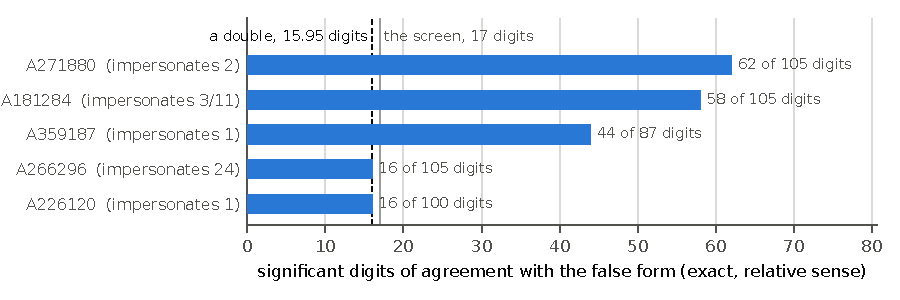
\includegraphics[width=0.74\linewidth]{fig/digits-not-evidence-depth.pdf}
\caption{Agreement depth of each audited constant's deepest false spelling, against the decimal reach of an IEEE~754 double (\DoubleDigits\ digits \cite{IEEE754}) and of the screen that admitted the constants to the exact stage. Drawn from the same re-run that writes Table~\ref{tab:imp}.}\label{fig:depth}
\end{figure}

Two of the five are the textbook shape of the failure. \texttt{A266296} is named by its contributor ``a number close to 24, related to the Ramanujan number $e^{\pi\sqrt{163}}$'': the near-integer phenomenon that made that constant famous reaches \RamDepth\ digits here and is refuted at \RamPublished. \texttt{A271880} is the probability that a random real number is evil; it agrees with $1/5$ to \EvilDepth\ of its \EvilPublished\ published digits, and with the decimal point placed as the name implies the difference from $1/5$ is about \EvilGapProb\ (OEIS records it as \texttt{A271881}, as the family's source notes record). A screen at any depth below sixty digits calls this constant $1/5$; the inequality \eqref{eq:exact} does not. None of this surprises the contributors who entered these constants; the point is what a screen does with them.


\subsection{Calibration and controls}\label{sec:calib}

An instrument that can refute must be shown not to refute truths. The engine battery \cite{repo} holds \CalibCount\ constants whose closed forms are known ($\pi$, $e$, $\sqrt2$, $\varphi$, $\ln2$, $\sqrt3$, $4\pi$, $\pi/4$) and requires that each keeps its form through the screen: zero false refutations is a gate, and it once fired. The first screen used 25 digits, a width of $10^{-24}$ in doubles whose spacing near $1.4$ is $2.2\times10^{-16}$; the interval collapsed to a single double and the engine refuted $\sqrt2$ as the closed form of the decimal expansion of $\sqrt2$. The present \ScreenDigits\ digits with \ScreenUlps\ ulps of outward padding are the repair, and the battery plants the failure too: an enclosure deliberately shifted off $\sqrt2$ must refute it. A second control guards the other direction: \texttt{A019762}, named ``Decimal expansion of 2*e'', was once certified as a discovery because a name regex missed the asterisk; it must never be a hit again.

\section{Part II: the Ramanujan Machine's sheets as a standing registry}

\subsection{The corpus: seven sheets, pinned by their bytes}\label{sec:sheets}

The Machine publishes its results as PDF sheets \cite{RMsheets}. Seven are held in the repository with their SHA-256 digests recorded, and every certificate re-hashes its sheet before it decides anything: a certificate is over a byte sequence, and a sheet whose bytes drift refuses every row transcribed from it (Table~\ref{tab:pins}). The five tables of 2020--2022 ($\zeta(3)$, Catalan's $G$, $\pi^2$, $\ln2$, mixed orders of $\zeta$) are transcribed row for row, \TableRows\ rows, re-counted from the pinned bytes at every run of the tool that writes this note. The two 2018 sheets ($e$ and $\pi$) print \EDisplays\ and \PiDisplays\ formula displays, many of them sign variants of one another, and the registry holds \ERows\ and \PiRows\ distinct continued fractions from them, those that normalise to positive continued fractions. The Machine's results page lists \RmListed\ sheet files as of the repository's last sweep (\RmSweepDate); \RmOutside\ of them (\RmOutsideList) are not in the registry. The registry is therefore complete for the five tables and partial for the 2018 sheets, and the counts below are counts of \emph{registry rows}, \RmPrinted\ in all.

\begin{table}[t]\centering\footnotesize
\begin{tabular}{lrrl}\toprule
sheet & rows or displays printed & rows in the registry & SHA-256 of the pinned file \\\midrule
\PinRows
\bottomrule\end{tabular}
\caption{The seven pinned sheets. The first count is the number of Novelty-labelled rows in the pinned PDF, or, for the two 2018 sheets, of formula displays.}\label{tab:pins}
\end{table}

A row of the registry is a continued fraction together with a claimed closed form; the continued fraction is the mathematical object and is what the audit decides. In the sheets' own labelling, a row is
\[
a_0+\cfrac{b_1}{a_1+\cfrac{b_2}{a_2+\cdots}},\qquad a_n,b_n\in\mathbb Z[n],
\]
with $a(n)$ the partial denominators and $b(n)$ the partial numerators; for every row of the five tables $a_0=a(0)$, and for the 2018 rows $a_0$ is stated in Table~\ref{tab:regA}. All rows but the 2018 ones and two $\pi^2$ rows have $b_n<0$ (minus continued fractions). Distinct rows may claim one value: \RmSameValuePairs\ pairs of registry rows do (\RmSameValueList), and they are distinct conjectures, each decided on its own enclosure.

\subsection{The decision procedure}\label{sec:method}

\paragraph{Positive continued fractions.}
\begin{lemma}[proved seed]\label{lem:seed}
Let $a_n>0$ and $b_n\ge1$ for all $n\ge1$, and let $t_{N+1}=a_{N+1}/(b_{N+1}+a_{N+2}/(b_{N+2}+\cdots))$ be the tail from level $N+1$ of a convergent positive continued fraction. Then $t_{N+1}\in(0,\,a_{N+1}/b_{N+1}]$.
\end{lemma}
\begin{proof}
The quantity added to $b_{N+1}$ in the denominator is nonnegative, and the tail is positive.
\end{proof}
Backward interval iteration $T\leftarrow a_n/(b_n+T)$ from the seed interval, with outward rounding at every operation \cite{MKC09,Tu11}, encloses the value of the whole fraction; the instrument verifies positivity and exact representability ($|a_n|,|b_n|<2^{53}$) over the range it uses and refuses otherwise. (The instrument's own notation exchanges $a$ and $b$; the tables of this note use the sheets' labelling.)

\paragraph{Minus continued fractions.}\label{sec:minus}
For $x=b_0-a_1/(b_1-a_2/(b_2-\cdots))$ with $a_n,b_n>0$ (the instrument's notation, in which the sheets' $b_n$ is $-a_n$), Lemma~\ref{lem:seed} does not apply: a subtraction can take a tail anywhere. The certificate replaces the seed by a proved band. Write the tail from level $n$ as $s_n=b_n-a_{n+1}/s_{n+1}$, so that $x=b_0-a_1/s_1$, and let the certificate name two polynomials $L(n),U(n)\in\mathbb Q[n]$ and a base index $N_0$.

\begin{lemma}[tail band]\label{lem:band}
Suppose that for all integers $n\ge N_0$,
\begin{align*}
&\text{(T)}\quad L(n)\le b_n\le U(n),\qquad\qquad\text{(P)}\quad L(n)>0,\ a_n>0,\\
&\text{(I$-$)}\quad b_n-\frac{a_{n+1}}{L(n+1)}\ge L(n),\qquad\ \text{(I$+$)}\quad b_n-\frac{a_{n+1}}{U(n+1)}\le U(n).
\end{align*}
Then for every depth $k\ge n\ge N_0$ the depth-$k$ truncation $s^{(k)}_n$ (with $s^{(k)}_k=b_k$) lies in $[L(n),U(n)]$. Consequently the backward interval iteration seeded with $[L(N+1),U(N+1)]$, outward-rounded, encloses the convergent $x_k$ for every $k\ge N+1$; the convergents $x_k$ decrease strictly in $k$, are bounded below by the enclosure's lower end, hence converge, and their limit lies in the closed enclosure.
\end{lemma}
\begin{proof}
By (T) the terminal value lies in the band. Each map $f_n(t)=b_n-a_{n+1}/t$ is increasing for $t>0$, so (I$-$) and (I$+$) carry the band down one level: if $s^{(k)}_{n+1}\in[L(n+1),U(n+1)]$ then $s^{(k)}_n=f_n(s^{(k)}_{n+1})\in[f_n(L(n+1)),f_n(U(n+1))]\subseteq[L(n),U(n)]$; finite induction from $n=k$ gives containment at every level, and the interval iteration from the seed then encloses $s^{(k)}_1$ and $x_k$ for every $k\ge N+1$ at once. Comparing depths $k$ and $k+1$, the terminal drops ($b_k-a_{k+1}/b_{k+1}<b_k$) and increasing maps propagate the drop, so $x_k$ is strictly decreasing and bounded below by the enclosure; it converges, and the limit lies in the closed enclosure. No convergence theorem is consumed.
\end{proof}

The four families of inequalities are polynomial in $n$, and each is proved for all integers $n\ge N_0$ by \emph{shift-and-check}: substitute $n=N_0+m$, expand exactly over rational coefficients (after clearing the positive denominators $L(n+1)$, $U(n+1)$), and require every coefficient of the polynomial in $m$ to be nonnegative. The check is sufficient and not necessary; a certificate that fails it is refused, never patched. The maps $f_n$ need a fixed sign of $t$ rather than positivity, and for the finitely many levels below $N_0$ the interval iteration certifies sign-definiteness directly: some Catalan rows have genuinely negative head tails and are decided this way, while an interval containing zero refuses the row.

\paragraph{The constants.}
\begin{lemma}[$\zeta(s)$ from its series]\label{lem:zeta}
For an integer $s\ge2$ and $K\ge1$, with $S_K=\sum_{k\le K}k^{-s}$ summed exactly,
\[
S_K+\frac{2^{s-1}}{(s-1)(2K+1)^{s-1}}-\frac{s\,2^{s-2}}{3\,(2K-1)^{s+1}}\;\le\;\zeta(s)\;\le\;S_K+\frac{2^{s-1}}{(s-1)(2K+1)^{s-1}} .
\]
\end{lemma}
\begin{proof}
$x^{-s}$ is convex, so $k^{-s}\le\int_{k-1/2}^{k+1/2}x^{-s}\,dx$ (the tangent at $k$ lies below the curve), and summing over $k>K$ gives the upper bound $\int_{K+1/2}^\infty x^{-s}dx$. The midpoint rule on each cell errs by at most $\max f''/24=s(s+1)(k-1/2)^{-s-2}/24$, and $\sum_{k>K}(k-1/2)^{-s-2}\le\int_{K-1/2}^\infty x^{-s-2}dx$, which gives the lower bound.
\end{proof}
At $s=3$, $K=\ZetaThreeK$ the bracket has width \ZetaThreeWidth\ and its ends, rounded, are $\ZetaThreeLo$ and $\ZetaThreeHi$; at $K=\ZetaHighK$ the brackets for $\zeta(5)$ and $\zeta(7)$ have widths \ZetaFiveWidth\ and \ZetaSevenWidth. Both ends are exact rationals. Catalan's constant is bracketed from its alternating series with the tail bounded by the alternating-series estimate, which needs $1/(2k+1)^2$ to be convex; the convexity is a polynomial identity, the second difference expanding to $\CatalanConvexity$ with every coefficient positive, re-derived at every certification (width \CatalanWidth). $\pi^2$ and $\ln2$ come from certified arbitrary-precision enclosures (widths \PiSqWidth\ and \LnTwoWidth); $\zeta(2)=\pi^2/6$ and $\zeta(4)=\pi^4/90$ are Euler's proved identities, consumed and named, and the battery holds the series route of Lemma~\ref{lem:zeta} and the $\pi$ route in mutual containment. The one two-constant form on the sheets, $8G-\pi\operatorname{arcosh}2$, is bracketed factor by factor (width \CatalanEWidth).

\paragraph{The comparison.}
A claimed form on the 2020--2022 sheets is M\"obius in one constant, $(p+qK)/(s+tK)$, or, on the mixed-orders sheet, $p/(c_0+\sum c_i\zeta(s_i))$; its exact bracket is formed from the constant's bracket by sign-aware endpoint selection, and a denominator interval containing zero refuses the row. The enclosure of the continued fraction, two doubles, is converted losslessly to rationals (every double is $m\cdot2^e$); the verdict is \vR\ when the two brackets are disjoint and \vS\ otherwise, with the width reported. Three $\pi^2$ rows have a negative first partial numerator; exact algebra moves the head aside ($x=a_0+c/y$ turns the claimed form into a M\"obius form for $y$), and deciding $y$ decides $x$.

\subsection{The $\zeta(3)$ sheet}\label{sec:zeta3}

The $\zeta(3)$ sheet has five rows: three known identities, among them Ap\'ery's continued fraction for $6/\zeta(3)$ \cite{Ap79,vdP79,Zu02}, and two the sheet marks new and unproven. All five \vS\ (Table~\ref{tab:zeta3}). For Ap\'ery's row the certificate is $N_0=\AperyNZero$, $L=\AperyL$, $U=\AperyU$, depth \AperyDepth, and the checker reports six proved facts, each by shift-and-check: $a(n)>0$ for $n\ge1$, $L(n)>0$, (T) in both directions, (I$-$) and (I$+$), the last five for all $n\ge\AperyNZero$. The two flagged rows are enclosed as tightly as the known ones; what \emph{unproven} means on the sheet is that no proof is on record, not that the numerics are weaker.

\begin{table}[t]\centering\scriptsize\setlength{\tabcolsep}{4pt}
\begin{tabular}{llllll}\toprule
row & status & claimed form & certified enclosure & width & depth \\\midrule
\ZetaThreeRows
\bottomrule\end{tabular}
\caption{The $\zeta(3)$ sheet, decided. \ZetaThreePosRow\ is the positive continued fraction (Lemma~\ref{lem:seed}); the others are decided by tail bands (Lemma~\ref{lem:band}). The enclosure is printed to fifteen decimals; the exact comparison uses the full doubles. Status is the sheet's own label.}\label{tab:zeta3}
\end{table}

One row hides a trap worth recording. The row for $1/\zeta(3)$ has $a_n=n^3+(n+1)^3$ and $b_n=-n^6$ (sheet labelling), that is $a_{n}=n^6$, $b_n=n^3+(n+1)^3$ in the instrument's.

\begin{lemma}[the spurious exact solution]\label{lem:spur}
The tail recursion $s_n=b_n-a_{n+1}/s_{n+1}$ of the $1/\zeta(3)$ row is solved exactly by $s_n=n^3$:
\[
n^3+(n+1)^3-\frac{(n+1)^6}{(n+1)^3}=n^3\quad\text{identically},
\]
and following this solution gives the continued fraction the value $0$, not $1/\zeta(3)$.
\end{lemma}
\begin{proof}
The displayed identity is $b(n)(n+1)^3-a(n+1)-n^3(n+1)^3\equiv0$ in $\mathbb Z[n]$; it is expanded and cancelled monomial by monomial at every build of this note (the macro file records that it \SpuriousIdentity). With $s_1=1$ the value is $b_0-a_1/s_1=1-1=0$.
\end{proof}

The spurious solution sits against the true branch: the fixed-point equation of the leading orders, $c^2-2c+1=0$, has a double root. A band whose lower edge is $n^3$ passes the four checks of Lemma~\ref{lem:band} with equality in (I$-$) and encloses nothing useful; the certificate uses $L=\InvBandL$, $U=\InvBandU$, $N_0=1$, and Table~\ref{tab:invband} records what the checker and the evaluator say about $L=n^3+cn^2$ for $c=0,\dots,3$ at depth \InvProbeDepth\ ($c=\InvBandC$ is the largest integer admitted). The continued fraction genuinely converges slowly (the per-level contraction is $1-O(1/n)$), so the certified width at depth \InvDepth\ is honestly \InvWidth, while every fast row of the sheet reaches machine precision by depth \FastDepth. The same double root governs all five rows of the mixed-orders sheet (Section~\ref{sec:refuted}). The sheet also taught the registry a lesson about transcription: re-read against the pinned bytes, the audit was found to be running on four rows of a five-row table, the missing row $5/(2\zeta(3))$ being the one positive continued fraction in the table.

\begin{table}[t]\centering\footnotesize
\begin{tabular}{lp{10.5cm}}\toprule
$L(n)$ & the checker, then the evaluator at depth \InvProbeDepth\ ($U(n)=b(n)$, $N_0=1$) \\\midrule
\InvBandRows
\bottomrule\end{tabular}
\caption{Lower bands for the $1/\zeta(3)$ row. The band at the spurious solution is certified and evaluates to nothing; the certificate's $c=\InvBandC$ is the largest integer admitted.}\label{tab:invband}
\end{table}

\subsection{The registry}\label{sec:registry}

Tables~\ref{tab:regA} and \ref{tab:regB} list every registry row with its defining polynomials, the claimed form, the verdict and the enclosure width; Figure~\ref{fig:widths} draws the widths by sheet. The widest surviving enclosure is \RmWidest\ (\RmWidestId, $\RmWidestForm$), so the survivals are not near misses: at those widths a false row would be refuted (Section~\ref{sec:controls}). The status column is provenance, what the sheet printed at publication; rows proved since keep the sheet's label, and the registry records separately what has been offered as a proof (two $\pi^2$ rows the sheet itself marks proven, citing \cite{KO21}; a 2026 preprint offered for \cf{rm-z3-new2} \cite{Sh26}, not verified here).

\begin{table}[!t]\centering\footnotesize\setlength{\tabcolsep}{3.5pt}
\resizebox{\linewidth}{!}{\begin{tabular}{llllllr}\toprule
row & status & $a(n)$ & $b(n)$ & claimed form & verdict & width \\\midrule
\RegistryRowsA
\bottomrule\end{tabular}}
\caption{The registry, part one: the 2018, $\zeta(3)$, $\ln2$ and mixed-orders sheets. Status: \emph{known}; \emph{unproven} (the sheet's ``new and unproven''); \emph{printed} (row 3 as printed); \emph{ours} (our correction, not a printed row). $a_0=a(0)$ except for the 2018 rows, \RmTwoKLeading, where ``$1;$'' is the first partial numerator and the polynomial holds for $n\ge2$.}\label{tab:regA}
\end{table}

\begin{table}[!t]\centering\footnotesize\setlength{\tabcolsep}{3.5pt}
\resizebox{\linewidth}{!}{\begin{tabular}{llllllr}\toprule
row & status & $a(n)$ & $b(n)$ & claimed form & verdict & width \\\midrule
\RegistryRowsB
\bottomrule\end{tabular}}
\caption{The registry, part two: the Catalan and $\pi^2$ sheets, $a_0=a(0)$ throughout. Status tags as in Table~\ref{tab:regA}; \emph{proven} is the sheet's ``new and proven'', citing \cite{KO21}.}\label{tab:regB}
\end{table}

\begin{figure}[!t]\centering
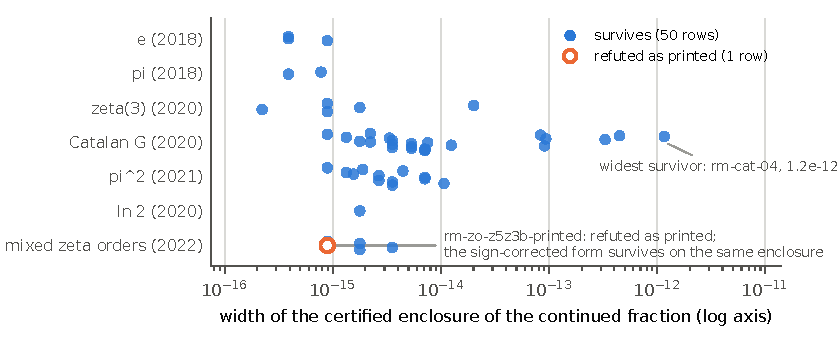
\includegraphics[width=0.68\linewidth]{fig/digits-not-evidence-widths.pdf}
\caption{The \RmPrinted\ printed registry rows by sheet, each at the width of its certified enclosure; the one refuted row is drawn hollow and named.}\label{fig:widths}
\end{figure}

\subsection{The refuted row}\label{sec:refuted}

The July 2022 sheet prints five rows, all new and unproven, all with $b_n=-n^{2k}$ and $\deg a=k$, so that the leading orders of every tail recursion give the double root of Lemma~\ref{lem:spur}. The tail ansatz $s_n=n^k+\alpha n^{k-1}+\cdots$ leaves $\alpha$ undetermined at first order and fixed at second order by the quadratic $\alpha^2-(k-1)\alpha+\big(\binom k2-a_{k-2}\big)=0$, $a_{k-2}$ the coefficient of $n^{k-2}$ in $a(n)$; for the five rows it factors over $\mathbb Z$ (Table~\ref{tab:branch}, re-factored at every build), and the band $L(n)=n^k+\alpha_+n^{k-1}$ at the larger root, with $U=a(n)$ and $N_0=1$, passes the four checks; the band at the smaller root fails (I$-$), a planted control.

\begin{table}[t]\centering\footnotesize
\begin{tabular}{llllll}\toprule
row & $k$ & the quadratic in $\alpha$ & factored & band $L(n)$ & width \\\midrule
\BranchRows
\bottomrule\end{tabular}
\caption{The mixed-orders sheet: each row's sub-leading quadratic, its integer roots, and the certified band.}\label{tab:branch}
\end{table}

The third row prints the identity $2/(2\zeta(5)-2\zeta(3)-1)=\text{CF}$ with $a_n=n^5+(n+1)^5+6(n^3+(n+1)^3)-4(2n+1)$ and $b_n=-n^{10}$. Expanding the printed $a_n$ gives $\RowThreePoly$ (checked at every build against the transcription), so $a_1=\RowThreeAOne$; the printed convergent display shows $a_1=\RowThreePrintedAOne$, which contradicts the row's own polynomial, and the displays of the rows with $b_n=-n^{10}$ and $-n^{14}$ reuse the $n^8$ numerators of the first row. The polynomial column is the object, and it is what the audit decides. From the band of Table~\ref{tab:branch} at depth \RowThreeDepth\ the continued fraction lies in
\[
\RowThreeEnclosure\qquad\text{(width \RowThreeWidth)},
\]
while $2/(2\zeta(5)-2\zeta(3)-1)$, bracketed from Lemma~\ref{lem:zeta}, is $\RowThreePrintedValue\ldots$: negative, and the printed identity is false. The sheet contains at least three typographic errors, and one of them makes a printed identity false. The underlying computation appears to have been right: the exact bracket of $2/(2\zeta(5)-2\zeta(3)+1)$ (width \RowThreeCorrFormWidth) meets the same enclosure, which is Proposition~\ref{prop:corr}. The two decisions are recorded as two rows sharing one continued fraction; the battery requires the printed row to be refuted with the mechanism named and the corrected row to survive on the identical enclosure, and a row expected to refute that does not is refused by name rather than recorded either way.

As of 2026-08-27 the repository's sweep of the Machine's results pages, its public repositories and arXiv found no earlier refutation of a printed Ramanujan Machine row on record; the sweep re-runs each session (last on \RmSweepDate), and if an earlier erratum surfaces this sentence is withdrawn, the mathematics being unchanged. The sheets mark these rows as conjectures by construction; the finding here is that the search worked and the print slipped.

\subsection{Controls}\label{sec:controls}

The continued-fraction instrument's battery runs \CfBatteryPass\ checks at every test of the repository and before this note's numbers are written; \CfBatteryRed\ of them are planted failures that must fire: a form displaced from $\pi/4$ by $10^{-6}$ against Brouncker's fraction, the false form $1/\zeta(3)$ against the row that claims $8/(7\zeta(3))$, and a forged $3/(5G)$ against a Catalan row must be \vR; a negative partial numerator, a coefficient past $2^{53}$, a band that excludes the tail, a band that violates (I$-$), a nonpositive $a(n)$, a form whose denominator interval contains zero, a head interval containing zero, and the spurious-branch band of the mixed-orders sheet must each be \vF\ with the reason. The calibrations are Brouncker's $\pi/4$, Euler's $e-1$, Ap\'ery's $6/\zeta(3)$, the two $\pi^2$ rows the sheet marks proven, and the known rows: an evaluator that refuted proved mathematics would be broken, and the battery would say so before any verdict on an unproven row were recorded.

\section{The common lesson}

The two parts are one experiment seen from both ends. In Part~I, published digit streams agree with false closed forms to depths no floating-point screen reaches, and a probability argument from the depth of agreement cannot tell them from identities; one integer inequality can. In Part~II, each printed conjecture is decided against an enclosure whose every ingredient is proved inside the certificate, with three outcomes rather than a confidence. What the two share is what matters for announcements of machine-found mathematics.
\begin{itemize}\setlength{\itemsep}{1pt}
\item \emph{The object is published, not only the value.} A continued fraction is its polynomials; a constant is its digit stream and its offset. The one row refuted here was refutable because its polynomials were printed.
\item \emph{The comparison is exact, and refusal is a verdict.} Doubles enter only as enclosure ends and are converted losslessly; a tail interval touching zero, a form whose denominator may vanish, a band that fails a check, a source whose bytes have drifted, each refuses with its reason and is counted on neither side. A pipeline that cannot refuse is indistinguishable from one that mints false positives.
\item \emph{Survival is a width, not a proof.} Fifty rows survive at widths between \RmNarrowest\ and \RmWidest; equality is open for each, and the registry says so in the arithmetic that refuted the fifty-first.
\item \emph{The record is a registry.} Verdicts are recomputed from pinned bytes at every build; a new sheet is new corpus; a later proof changes a status, not a verdict.
\end{itemize}
A digit count supplies none of these. It is a fine way to find candidates, and it is how every row in the registry was found; it is not evidence that any of them is true.

\section{What is not claimed}

\begin{itemize}\setlength{\itemsep}{1pt}
\item No identity is proved. \vS\ certifies consistency to the stated width and nothing more; the \RmSurvive\ surviving rows remain conjectures except where the literature has proved them, and the registry does not adjudicate the proofs it records as offered \cite{KO21,Sh26}.
\item The refutations of Part~I are conditional on the OEIS digit streams being correct and are refutations up to a power of ten; nothing is claimed about the five constants beyond their not being the listed rationals. The vocabulary is small (\FormsTested\ positive spellings) and only its rational values reach the exact stage. The audit found \OeisHits\ discoveries and claims none.
\item The registry is complete for the five 2020--2022 tables and partial for the two 2018 sheets, whose \EDisplays\ and \PiDisplays\ displays contribute \ERows\ and \PiRows\ rows; \RmOutside\ files on the Machine's results page are outside it. ``Every row'' in this note means every registry row.
\item The refuted row is refuted \emph{as printed}: a claim about the sheet's print, not about the Machine's search, whose output the corrected identity appears to be; the three typographic errors are a reading of the pinned PDF. The priority sentence of Section~\ref{sec:refuted} is a dated statement about a sweep, not a claim of novelty for the mathematics, which is elementary and surely known. Nothing is claimed about the Machine's algorithms or its paper \cite{RM21}; the sheets are audited as published documents, and the reading of its methodology as a collision-probability argument is the registry page's, recorded there \cite{repo}.
\end{itemize}

\cmrepro{{\sloppy Part~I: \texttt{families/\allowbreak oeis-closedform.js} over \texttt{corpus/\allowbreak oeis-constants.json} (\OeisSource, fetched \OeisPinned) and \texttt{corpus/\allowbreak survivors-confirmed.json}; the catalog is recomputed by \texttt{tools/\allowbreak build-report-impostors.js}, the calibration by \texttt{tools/\allowbreak test-engine.js}. Part~II: \texttt{families/\allowbreak ramanujan-audit.js} over the seven sheets in \texttt{corpus/sources/} pinned in \texttt{PINS.json}, with \texttt{instruments/\allowbreak cf/} and \texttt{instruments/\allowbreak bigfloat/\allowbreak constants.js}; \texttt{node instruments/\allowbreak cf/\allowbreak battery.js} re-certifies the registry with its \CfBatteryRed\ planted controls in seconds; \texttt{tools/\allowbreak build-report-rm-audit.js} and \texttt{tools/\allowbreak build-report-zeta3.js} rebuild the registry pages \cite{repo}. The macros and figures of this note are written by \texttt{node tools/\allowbreak paper-numbers/\allowbreak digits-not-evidence.js} \texttt{--figs}, which re-runs both families (about \ImpSeconds\ and \RmSeconds\ seconds), the battery, the polynomial identities and the row counts from the pinned bytes, and refuses when a record no longer supports a sentence; repository commit \RepoCommit.\par}}

\begin{thebibliography}{99}\footnotesize\setlength{\itemsep}{0pt}
\bibitem{BB04} J.~M. Borwein, D.~H. Bailey, \emph{Mathematics by Experiment: Plausible Reasoning in the 21st Century}, A K Peters, 2004.
\bibitem{FBA99} H.~R.~P. Ferguson, D.~H. Bailey, S. Arno, Analysis of PSLQ, an integer relation finding algorithm, Math.\ Comp.\ 68 (1999) 351--369.
\bibitem{LLL82} A.~K. Lenstra, H.~W. Lenstra Jr., L. Lov\'asz, Factoring polynomials with rational coefficients, Math.\ Ann.\ 261 (1982) 515--534.
\bibitem{RM21} G. Raayoni, S. Gottlieb, Y. Manor, G. Pisha, Y. Harris, U. Mendlovic, D. Haviv, Y. Hadad, I. Kaminer, Generating conjectures on fundamental constants with the Ramanujan Machine, Nature 590 (2021) 67--73.
\bibitem{RMsheets} The Ramanujan Machine, result sheets, \url{https://www.ramanujanmachine.com/idea/results/}; the seven files audited here are pinned by SHA-256 in \cite{repo} (Table~\ref{tab:pins}).
\bibitem{OEIS} OEIS Foundation Inc., \emph{The On-Line Encyclopedia of Integer Sequences}, \url{https://oeis.org}; bulk files \texttt{names.gz} and \texttt{stripped.gz} as fetched on \OeisPinned.
\bibitem{IEEE754} IEEE Std 754-2019, IEEE Standard for Floating-Point Arithmetic, IEEE, 2019.
\bibitem{Ap79} R. Ap\'ery, Irrationalit\'e de $\zeta(2)$ et $\zeta(3)$, Ast\'erisque 61 (1979) 11--13.
\bibitem{vdP79} A. van der Poorten, A proof that Euler missed\ldots\ Ap\'ery's proof of the irrationality of $\zeta(3)$, Math.\ Intelligencer 1 (1979) 195--203.
\bibitem{Zu02} W. Zudilin, An elementary proof of Ap\'ery's theorem, arXiv:math/0202159, 2002.
\bibitem{MKC09} R.~E. Moore, R.~B. Kearfott, M.~J. Cloud, \emph{Introduction to Interval Analysis}, SIAM, 2009.
\bibitem{Tu11} W. Tucker, \emph{Validated Numerics: A Short Introduction to Rigorous Computations}, Princeton University Press, 2011.
\bibitem{KO21} arXiv:2103.03554 (Kadyrov and Orynbassar), the proof the Machine's $\pi^2$ sheet cites for its two ``new and proven'' rows, as recorded in the registry \cite{repo}; not independently verified here.
\bibitem{Sh26} arXiv:2604.06239, offered as a proof of the identity $12/(7\zeta(3))$ of row \cf{rm-z3-new2}, as recorded in the repository's claim sweep \cite{repo}; not verified here.
\bibitem{repo} C. Toledo, \emph{cert-machine: independent exact certification of machine-generated mathematics}, repository and Zenodo archive, doi:10.5281/zenodo.22225860; the report pages \texttt{impostors}, \texttt{rm-audit} and \texttt{zeta3-audit} under \url{https://carlostoledo.co/reports/}.
\end{thebibliography}

\end{document}
